%%%GKA_PR_template.tex

\documentclass[a4paper]{article}
\usepackage{praktikum}
\begin{document}
	
%%
%% Bitte das Deckblatt nicht verändern


\thispagestyle{empty}
\begin{center}

    {\large {\bf   BAI3-GKA WiSe2§ \\ Graphentheoretische Konzepte und Algorithmen \\[5mm]} }
    
{\huge Praktikumsaufgabe-Template  \\[5mm] Deckblatt}\\

\end{center}

				\begin{tabular}[t]{|r|l|}
				 \hline
%%%%				
%%%% Bitte  Ihren Namen und  Ihr Team und die Gruppe angeben
				GKA-Gruppe&                 \raisebox{-3mm}{\rule[8mm]{100mm}{0mm} }\\ \hline    
				Team &                                                        \\ \hline			
				& \textit{Iryna Trygub }               \\ \hline    
				& \textit{Ansgar Deuschel }               \\ \hline			
				& \textit{Kristoffer Schaaf }             \\ \hline  			
				\multicolumn{2}{c}{}\\  			
				\multicolumn{2}{l}{Bearbeitete Themen in Stichpunkten:}\\			
				\multicolumn{2}{c}{}\\  \hline
				Iryna Trygub &              \\ \hline    
				Ansgar Deuschel &                \\ \hline			
				Kristoffer Schaaf & Ops            \\ \hline 		
				\multicolumn{2}{c}{}\\  			
				\multicolumn{2}{l}{Geschätzte Arbeitszeiten in Stunden:}\\			
				\multicolumn{2}{c}{}\\  \hline
				Iryna Trygub &               \\ \hline    
				Ansgar Deuschel &                \\ \hline			
				Kristoffer Schaaf &               \\ \hline 			
				\end{tabular}
~\\[4mm]
		
		
\vfill


\newpage

\section{Einleitung}

\subsection{Vorab}

Angenommen, der Dijkstra Algorithmus wäre in zwei Ansätzen zu lösen. Dann wären der erste Ansatz, dass es einen Typ Kante gibt, in welchem die Vor- und Nachfolgenden Knoten und die Länge der jeweiligen Kante gespeichert werden.\\
Diese Kanten würde dann den Graphen bilden und diesen in Form eines Sets darstellen:\\$Set <Kante> graph = new\ HashSet<>()$.\\
Problematisch wird es jetzt allerdings schon, wenn der Startknoten gefunden werden soll. Hat dieser immer den Grad 1, können wir über das Set graph iterieren und stoppen, sobald der gesuchte Knoten in einer der Kanten enthalten ist. Ist der Grad des Startknoten allerdings größer 1, so muss über alle Kanten iteriert werden ob diese nicht mit dem Startknoten verbunden sind. Somit wäre schon der Start des Algorithmus ineffizient.

Der zweite Ansatz auf welchem auch folgende Implementierung\footnote{\url{https://github.com/eugenp/tutorials/blob/master/algorithms-modules/algorithms-miscellaneous-2/src/main/java/com/baeldung/algorithms/ga/dijkstra/Node.java}} basiert wäre, die Kante als solches zu abstrahieren und nicht als eigenen Typen zu implementieren. Es gäbe dann nur den Typen Knoten, welcher alle benachbarten Knoten mit zugehöriger Distanz enthält.\\
Auch diese Knoten können nun in einem Set gespeichert werden:\\
$Set<Knoten> graph = new\ HashSet<>()$.\\
Allerdings wird bei der Suche nach dem Startknoten die Iteration gestoppt, sobald dieser gefunden wurde.
Somit ist der zweite Ansatz vorerst effizienter.

\subsection{Aufbau des Graphen}

Um den Dijkstra Algorithmus innerhalb eines Graphen anwenden zu können, muss zuerst ein Graph aufgebaut werden.
Wie im vorherigen Kapitel beschrieben, genügt es ein Set mit Knoten zu definieren.
Die Knoten des Graphen müssen folgende Informationen enthalten: Einen eindeutigen, im Graphen nur einmal vorkommenden, Namen und die adjazenten Knoten. Letztere werden in Form einer Map definiert, da so der Knoten mit inzidenter Kante und dessen Länge sinnvoll zusammen gespeichert wird.

Bedingungen, welche für den Graphen gelten:
- Der Graph muss gewichtet sein und darf ausschließlich positive Kantengewichte haben
- Der Graph kann unendlich viele Knoten besitzen
- Allgemein kann Dijkstra auf einen gerichteten, ungerichteten oder gemischten Graphen angewendet werden. In dieser Implementierung wird aber ein ungerichteter Graph genutzt.

\subsection{Dijkstra Algorithmus in Worten}

Wie genau funktioniert der Dijkstra Algorithmus aber eigentlich und wo wird er angewendet?
Nehmen wir an Kreuzungen und Kreisverkehre seien Knoten und die Straßen, die diese verbinden die Kanten. Dann lässt sich bis auf Ausnahmen jedes Straßennetz durch einen Graphen darstellen. Um zu berechnen, wie Mensch am schnellsten von einem beliebigen Kreisverkehr zu einer beliebigen Kreuzung kommen kann, wird nur zum Beispiel der Dijkstra Algorithmus verwendet.

\begin{enumerate}
    \item Finden des Startknotens im Graphen.
    \item Dann die Distanz zu allen benachbarten Knoten berechnen und diese zusammen mit der Distanz zum Startknoten und den Knoten auf dem Weg dorthin in einer Open List speichern
    
    \item Nun den Knoten mit kürzester Distanz zum Startknoten in Open List suchen und Schritt 2 von diesem Knoten aus wiederholen
    \begin{enumerate}
        \item Wenn ein Knoten, welcher bereits in der Open List gespeichert ist, erneut besucht wird, wird verglichen ob die neue Distanz kürzer ist. Wenn ja, wird der Knoten inklusive der Distanz zum Startknoten und den Knoten auf dem Weg dorthin aktualisiert. Wenn die Distanz länger ist, wird der Weg verworfen.
        \item Wenn alle inzidenten Kanten eines Knotens bearbeitet wurden, wird dieser Knoten in die Closed List verschoben.
    \end{enumerate}

    \item Der Algorithmus ist beendet, wenn entweder
    \begin{enumerate}
        \item alle Knoten des Graphen besucht wurden oder
        \item die Distanz vom Start- zum Zielknoten, die bisher kleinste gefundene Distanz ist.
    \end{enumerate}
    
\end{enumerate}

\subsection{Elemente}

Die benötigten Elemente, bzw. Typen sind 

\section{Dokumentation Ihrer Implementierung}

\newpage

\cite{KN2012} 
und Ihre Abbildungen nicht, z.B. Abb.~\ref{fig:bild}.
  

\section{Beantwortung der  Fragen}
\begin{enumerate}
						\item Antwort auf die erste Frage
						\item 
					\end{enumerate}


\section*{Abbildungen}


\begin{figure}[h]
	\centering
		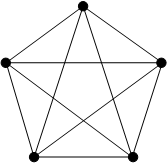
\includegraphics[width=0.50\textwidth]{Figs/Bild.png}		
	\caption{Beispiel für eine Abbildung}
	\label{fig:bild}
\end{figure}



\bibliographystyle{alpha}
\bibliography{mybib}
%%%%GKA_PR_template.tex

\documentclass[a4paper]{article}
\usepackage{praktikum}
\begin{document}
	
%%
%% Bitte das Deckblatt nicht verändern


\thispagestyle{empty}
\begin{center}

    {\large {\bf   BAI3-GKA WiSe2§ \\ Graphentheoretische Konzepte und Algorithmen \\[5mm]} }
    
{\huge Praktikumsaufgabe-Template  \\[5mm] Deckblatt}\\

\end{center}

				\begin{tabular}[t]{|r|l|}
				 \hline
%%%%				
%%%% Bitte  Ihren Namen und  Ihr Team und die Gruppe angeben
				GKA-Gruppe&                 \raisebox{-3mm}{\rule[8mm]{100mm}{0mm} }\\ \hline    
				Team &                                                        \\ \hline			
				& \textit{Iryna Trygub }               \\ \hline    
				& \textit{Ansgar Deuschel }               \\ \hline			
				& \textit{Kristoffer Schaaf }             \\ \hline  			
				\multicolumn{2}{c}{}\\  			
				\multicolumn{2}{l}{Bearbeitete Themen in Stichpunkten:}\\			
				\multicolumn{2}{c}{}\\  \hline
				Iryna Trygub &              \\ \hline    
				Ansgar Deuschel &                \\ \hline			
				Kristoffer Schaaf & Ops            \\ \hline 		
				\multicolumn{2}{c}{}\\  			
				\multicolumn{2}{l}{Geschätzte Arbeitszeiten in Stunden:}\\			
				\multicolumn{2}{c}{}\\  \hline
				Iryna Trygub &               \\ \hline    
				Ansgar Deuschel &                \\ \hline			
				Kristoffer Schaaf &               \\ \hline 			
				\end{tabular}
~\\[4mm]
		
		
\vfill


\newpage

\section{Einleitung}

\subsection{Vorab}

Angenommen, der Dijkstra Algorithmus wäre in zwei Ansätzen zu lösen. Dann wären der erste Ansatz, dass es einen Typ Kante gibt, in welchem die Vor- und Nachfolgenden Knoten und die Länge der jeweiligen Kante gespeichert werden.\\
Diese Kanten würde dann den Graphen bilden und diesen in Form eines Sets darstellen:\\$Set <Kante> graph = new\ HashSet<>()$.\\
Problematisch wird es jetzt allerdings schon, wenn der Startknoten gefunden werden soll. Hat dieser immer den Grad 1, können wir über das Set graph iterieren und stoppen, sobald der gesuchte Knoten in einer der Kanten enthalten ist. Ist der Grad des Startknoten allerdings größer 1, so muss über alle Kanten iteriert werden ob diese nicht mit dem Startknoten verbunden sind. Somit wäre schon der Start des Algorithmus ineffizient.

Der zweite Ansatz auf welchem auch folgende Implementierung\footnote{\url{https://github.com/eugenp/tutorials/blob/master/algorithms-modules/algorithms-miscellaneous-2/src/main/java/com/baeldung/algorithms/ga/dijkstra/Node.java}} basiert wäre, die Kante als solches zu abstrahieren und nicht als eigenen Typen zu implementieren. Es gäbe dann nur den Typen Knoten, welcher alle benachbarten Knoten mit zugehöriger Distanz enthält.\\
Auch diese Knoten können nun in einem Set gespeichert werden:\\
$Set<Knoten> graph = new\ HashSet<>()$.\\
Allerdings wird bei der Suche nach dem Startknoten die Iteration gestoppt, sobald dieser gefunden wurde.
Somit ist der zweite Ansatz vorerst effizienter.

\subsection{Aufbau des Graphen}

Um den Dijkstra Algorithmus innerhalb eines Graphen anwenden zu können, muss zuerst ein Graph aufgebaut werden.
Wie im vorherigen Kapitel beschrieben, genügt es ein Set mit Knoten zu definieren.
Die Knoten des Graphen müssen folgende Informationen enthalten: Einen eindeutigen, im Graphen nur einmal vorkommenden, Namen und die adjazenten Knoten. Letztere werden in Form einer Map definiert, da so der Knoten mit inzidenter Kante und dessen Länge sinnvoll zusammen gespeichert wird.

Bedingungen, welche für den Graphen gelten:
- Der Graph muss gewichtet sein und darf ausschließlich positive Kantengewichte haben
- Der Graph kann unendlich viele Knoten besitzen
- Allgemein kann Dijkstra auf einen gerichteten, ungerichteten oder gemischten Graphen angewendet werden. In dieser Implementierung wird aber ein ungerichteter Graph genutzt.

\subsection{Dijkstra Algorithmus in Worten}

Wie genau funktioniert der Dijkstra Algorithmus aber eigentlich und wo wird er angewendet?
Nehmen wir an Kreuzungen und Kreisverkehre seien Knoten und die Straßen, die diese verbinden die Kanten. Dann lässt sich bis auf Ausnahmen jedes Straßennetz durch einen Graphen darstellen. Um zu berechnen, wie Mensch am schnellsten von einem beliebigen Kreisverkehr zu einer beliebigen Kreuzung kommen kann, wird nur zum Beispiel der Dijkstra Algorithmus verwendet.

\begin{enumerate}
    \item Finden des Startknotens im Graphen.
    \item Dann die Distanz zu allen benachbarten Knoten berechnen und diese zusammen mit der Distanz zum Startknoten und den Knoten auf dem Weg dorthin in einer Open List speichern
    
    \item Nun den Knoten mit kürzester Distanz zum Startknoten in Open List suchen und Schritt 2 von diesem Knoten aus wiederholen
    \begin{enumerate}
        \item Wenn ein Knoten, welcher bereits in der Open List gespeichert ist, erneut besucht wird, wird verglichen ob die neue Distanz kürzer ist. Wenn ja, wird der Knoten inklusive der Distanz zum Startknoten und den Knoten auf dem Weg dorthin aktualisiert. Wenn die Distanz länger ist, wird der Weg verworfen.
        \item Wenn alle inzidenten Kanten eines Knotens bearbeitet wurden, wird dieser Knoten in die Closed List verschoben.
    \end{enumerate}

    \item Der Algorithmus ist beendet, wenn entweder
    \begin{enumerate}
        \item alle Knoten des Graphen besucht wurden oder
        \item die Distanz vom Start- zum Zielknoten, die bisher kleinste gefundene Distanz ist.
    \end{enumerate}
    
\end{enumerate}

\subsection{Elemente}

Die benötigten Elemente, bzw. Typen sind 

\section{Dokumentation Ihrer Implementierung}

\newpage

\cite{KN2012} 
und Ihre Abbildungen nicht, z.B. Abb.~\ref{fig:bild}.
  

\section{Beantwortung der  Fragen}
\begin{enumerate}
						\item Antwort auf die erste Frage
						\item 
					\end{enumerate}


\section*{Abbildungen}


\begin{figure}[h]
	\centering
		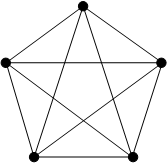
\includegraphics[width=0.50\textwidth]{Figs/Bild.png}		
	\caption{Beispiel für eine Abbildung}
	\label{fig:bild}
\end{figure}



\bibliographystyle{alpha}
\bibliography{mybib}
%%%%GKA_PR_template.tex

\documentclass[a4paper]{article}
\usepackage{praktikum}
\begin{document}
	
%%
%% Bitte das Deckblatt nicht verändern


\thispagestyle{empty}
\begin{center}

    {\large {\bf   BAI3-GKA WiSe2§ \\ Graphentheoretische Konzepte und Algorithmen \\[5mm]} }
    
{\huge Praktikumsaufgabe-Template  \\[5mm] Deckblatt}\\

\end{center}

				\begin{tabular}[t]{|r|l|}
				 \hline
%%%%				
%%%% Bitte  Ihren Namen und  Ihr Team und die Gruppe angeben
				GKA-Gruppe&                 \raisebox{-3mm}{\rule[8mm]{100mm}{0mm} }\\ \hline    
				Team &                                                        \\ \hline			
				& \textit{Iryna Trygub }               \\ \hline    
				& \textit{Ansgar Deuschel }               \\ \hline			
				& \textit{Kristoffer Schaaf }             \\ \hline  			
				\multicolumn{2}{c}{}\\  			
				\multicolumn{2}{l}{Bearbeitete Themen in Stichpunkten:}\\			
				\multicolumn{2}{c}{}\\  \hline
				Iryna Trygub &              \\ \hline    
				Ansgar Deuschel &                \\ \hline			
				Kristoffer Schaaf & Ops            \\ \hline 		
				\multicolumn{2}{c}{}\\  			
				\multicolumn{2}{l}{Geschätzte Arbeitszeiten in Stunden:}\\			
				\multicolumn{2}{c}{}\\  \hline
				Iryna Trygub &               \\ \hline    
				Ansgar Deuschel &                \\ \hline			
				Kristoffer Schaaf &               \\ \hline 			
				\end{tabular}
~\\[4mm]
		
		
\vfill


\newpage

\section{Einleitung}

\subsection{Vorab}

Angenommen, der Dijkstra Algorithmus wäre in zwei Ansätzen zu lösen. Dann wären der erste Ansatz, dass es einen Typ Kante gibt, in welchem die Vor- und Nachfolgenden Knoten und die Länge der jeweiligen Kante gespeichert werden.\\
Diese Kanten würde dann den Graphen bilden und diesen in Form eines Sets darstellen:\\$Set <Kante> graph = new\ HashSet<>()$.\\
Problematisch wird es jetzt allerdings schon, wenn der Startknoten gefunden werden soll. Hat dieser immer den Grad 1, können wir über das Set graph iterieren und stoppen, sobald der gesuchte Knoten in einer der Kanten enthalten ist. Ist der Grad des Startknoten allerdings größer 1, so muss über alle Kanten iteriert werden ob diese nicht mit dem Startknoten verbunden sind. Somit wäre schon der Start des Algorithmus ineffizient.

Der zweite Ansatz auf welchem auch folgende Implementierung\footnote{\url{https://github.com/eugenp/tutorials/blob/master/algorithms-modules/algorithms-miscellaneous-2/src/main/java/com/baeldung/algorithms/ga/dijkstra/Node.java}} basiert wäre, die Kante als solches zu abstrahieren und nicht als eigenen Typen zu implementieren. Es gäbe dann nur den Typen Knoten, welcher alle benachbarten Knoten mit zugehöriger Distanz enthält.\\
Auch diese Knoten können nun in einem Set gespeichert werden:\\
$Set<Knoten> graph = new\ HashSet<>()$.\\
Allerdings wird bei der Suche nach dem Startknoten die Iteration gestoppt, sobald dieser gefunden wurde.
Somit ist der zweite Ansatz vorerst effizienter.

\subsection{Aufbau des Graphen}

Um den Dijkstra Algorithmus innerhalb eines Graphen anwenden zu können, muss zuerst ein Graph aufgebaut werden.
Wie im vorherigen Kapitel beschrieben, genügt es ein Set mit Knoten zu definieren.
Die Knoten des Graphen müssen folgende Informationen enthalten: Einen eindeutigen, im Graphen nur einmal vorkommenden, Namen und die adjazenten Knoten. Letztere werden in Form einer Map definiert, da so der Knoten mit inzidenter Kante und dessen Länge sinnvoll zusammen gespeichert wird.

Bedingungen, welche für den Graphen gelten:
- Der Graph muss gewichtet sein und darf ausschließlich positive Kantengewichte haben
- Der Graph kann unendlich viele Knoten besitzen
- Allgemein kann Dijkstra auf einen gerichteten, ungerichteten oder gemischten Graphen angewendet werden. In dieser Implementierung wird aber ein ungerichteter Graph genutzt.

\subsection{Dijkstra Algorithmus in Worten}

Wie genau funktioniert der Dijkstra Algorithmus aber eigentlich und wo wird er angewendet?
Nehmen wir an Kreuzungen und Kreisverkehre seien Knoten und die Straßen, die diese verbinden die Kanten. Dann lässt sich bis auf Ausnahmen jedes Straßennetz durch einen Graphen darstellen. Um zu berechnen, wie Mensch am schnellsten von einem beliebigen Kreisverkehr zu einer beliebigen Kreuzung kommen kann, wird nur zum Beispiel der Dijkstra Algorithmus verwendet.

\begin{enumerate}
    \item Finden des Startknotens im Graphen.
    \item Dann die Distanz zu allen benachbarten Knoten berechnen und diese zusammen mit der Distanz zum Startknoten und den Knoten auf dem Weg dorthin in einer Open List speichern
    
    \item Nun den Knoten mit kürzester Distanz zum Startknoten in Open List suchen und Schritt 2 von diesem Knoten aus wiederholen
    \begin{enumerate}
        \item Wenn ein Knoten, welcher bereits in der Open List gespeichert ist, erneut besucht wird, wird verglichen ob die neue Distanz kürzer ist. Wenn ja, wird der Knoten inklusive der Distanz zum Startknoten und den Knoten auf dem Weg dorthin aktualisiert. Wenn die Distanz länger ist, wird der Weg verworfen.
        \item Wenn alle inzidenten Kanten eines Knotens bearbeitet wurden, wird dieser Knoten in die Closed List verschoben.
    \end{enumerate}

    \item Der Algorithmus ist beendet, wenn entweder
    \begin{enumerate}
        \item alle Knoten des Graphen besucht wurden oder
        \item die Distanz vom Start- zum Zielknoten, die bisher kleinste gefundene Distanz ist.
    \end{enumerate}
    
\end{enumerate}

\subsection{Elemente}

Die benötigten Elemente, bzw. Typen sind 

\section{Dokumentation Ihrer Implementierung}

\newpage

\cite{KN2012} 
und Ihre Abbildungen nicht, z.B. Abb.~\ref{fig:bild}.
  

\section{Beantwortung der  Fragen}
\begin{enumerate}
						\item Antwort auf die erste Frage
						\item 
					\end{enumerate}


\section*{Abbildungen}


\begin{figure}[h]
	\centering
		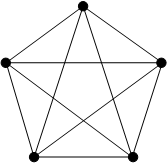
\includegraphics[width=0.50\textwidth]{Figs/Bild.png}		
	\caption{Beispiel für eine Abbildung}
	\label{fig:bild}
\end{figure}



\bibliographystyle{alpha}
\bibliography{mybib}
%%%%GKA_PR_template.tex

\documentclass[a4paper]{article}
\usepackage{praktikum}
\begin{document}
	
\input{deckblatt}
\newpage

\section{Einleitung}

\subsection{Vorab}

Angenommen, der Dijkstra Algorithmus wäre in zwei Ansätzen zu lösen. Dann wären der erste Ansatz, dass es einen Typ Kante gibt, in welchem die Vor- und Nachfolgenden Knoten und die Länge der jeweiligen Kante gespeichert werden.\\
Diese Kanten würde dann den Graphen bilden und diesen in Form eines Sets darstellen:\\$Set <Kante> graph = new\ HashSet<>()$.\\
Problematisch wird es jetzt allerdings schon, wenn der Startknoten gefunden werden soll. Hat dieser immer den Grad 1, können wir über das Set graph iterieren und stoppen, sobald der gesuchte Knoten in einer der Kanten enthalten ist. Ist der Grad des Startknoten allerdings größer 1, so muss über alle Kanten iteriert werden ob diese nicht mit dem Startknoten verbunden sind. Somit wäre schon der Start des Algorithmus ineffizient.

Der zweite Ansatz auf welchem auch folgende Implementierung\footnote{\url{https://github.com/eugenp/tutorials/blob/master/algorithms-modules/algorithms-miscellaneous-2/src/main/java/com/baeldung/algorithms/ga/dijkstra/Node.java}} basiert wäre, die Kante als solches zu abstrahieren und nicht als eigenen Typen zu implementieren. Es gäbe dann nur den Typen Knoten, welcher alle benachbarten Knoten mit zugehöriger Distanz enthält.\\
Auch diese Knoten können nun in einem Set gespeichert werden:\\
$Set<Knoten> graph = new\ HashSet<>()$.\\
Allerdings wird bei der Suche nach dem Startknoten die Iteration gestoppt, sobald dieser gefunden wurde.
Somit ist der zweite Ansatz vorerst effizienter.

\subsection{Aufbau des Graphen}

Um den Dijkstra Algorithmus innerhalb eines Graphen anwenden zu können, muss zuerst ein Graph aufgebaut werden.
Wie im vorherigen Kapitel beschrieben, genügt es ein Set mit Knoten zu definieren.
Die Knoten des Graphen müssen folgende Informationen enthalten: Einen eindeutigen, im Graphen nur einmal vorkommenden, Namen und die adjazenten Knoten. Letztere werden in Form einer Map definiert, da so der Knoten mit inzidenter Kante und dessen Länge sinnvoll zusammen gespeichert wird.

Bedingungen, welche für den Graphen gelten:
- Der Graph muss gewichtet sein und darf ausschließlich positive Kantengewichte haben
- Der Graph kann unendlich viele Knoten besitzen
- Allgemein kann Dijkstra auf einen gerichteten, ungerichteten oder gemischten Graphen angewendet werden. In dieser Implementierung wird aber ein ungerichteter Graph genutzt.

\subsection{Dijkstra Algorithmus in Worten}

Wie genau funktioniert der Dijkstra Algorithmus aber eigentlich und wo wird er angewendet?
Nehmen wir an Kreuzungen und Kreisverkehre seien Knoten und die Straßen, die diese verbinden die Kanten. Dann lässt sich bis auf Ausnahmen jedes Straßennetz durch einen Graphen darstellen. Um zu berechnen, wie Mensch am schnellsten von einem beliebigen Kreisverkehr zu einer beliebigen Kreuzung kommen kann, wird nur zum Beispiel der Dijkstra Algorithmus verwendet.

\begin{enumerate}
    \item Finden des Startknotens im Graphen.
    \item Dann die Distanz zu allen benachbarten Knoten berechnen und diese zusammen mit der Distanz zum Startknoten und den Knoten auf dem Weg dorthin in einer Open List speichern
    
    \item Nun den Knoten mit kürzester Distanz zum Startknoten in Open List suchen und Schritt 2 von diesem Knoten aus wiederholen
    \begin{enumerate}
        \item Wenn ein Knoten, welcher bereits in der Open List gespeichert ist, erneut besucht wird, wird verglichen ob die neue Distanz kürzer ist. Wenn ja, wird der Knoten inklusive der Distanz zum Startknoten und den Knoten auf dem Weg dorthin aktualisiert. Wenn die Distanz länger ist, wird der Weg verworfen.
        \item Wenn alle inzidenten Kanten eines Knotens bearbeitet wurden, wird dieser Knoten in die Closed List verschoben.
    \end{enumerate}

    \item Der Algorithmus ist beendet, wenn entweder
    \begin{enumerate}
        \item alle Knoten des Graphen besucht wurden oder
        \item die Distanz vom Start- zum Zielknoten, die bisher kleinste gefundene Distanz ist.
    \end{enumerate}
    
\end{enumerate}

\subsection{Elemente}

Die benötigten Elemente, bzw. Typen sind 

\section{Dokumentation Ihrer Implementierung}

\newpage

\cite{KN2012} 
und Ihre Abbildungen nicht, z.B. Abb.~\ref{fig:bild}.
  

\section{Beantwortung der  Fragen}
\begin{enumerate}
						\item Antwort auf die erste Frage
						\item 
					\end{enumerate}


\section*{Abbildungen}


\begin{figure}[h]
	\centering
		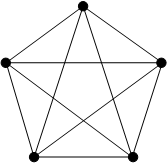
\includegraphics[width=0.50\textwidth]{Figs/Bild.png}		
	\caption{Beispiel für eine Abbildung}
	\label{fig:bild}
\end{figure}



\bibliographystyle{alpha}
\bibliography{mybib}
%\include{GKA_PR_template.bbl}

\end{document}

\end{document}

\end{document}

\end{document}